\documentclass[aps,prl,twocolumn,superscriptaddress,showpacs,amsmath,amssymb]{revtex4-2}

% Packages
\usepackage[utf8]{inputenc}
\usepackage[T1]{fontenc}
\usepackage{textcomp}
\usepackage{mathtools, extarrows}
\usepackage[colorlinks,linkcolor=blue,citecolor=red,urlcolor=blue,bookmarks=true]{hyperref}
\usepackage{subcaption}
\usepackage{xcolor}
\usepackage{graphicx}% Include figure files
\usepackage{import}
\usepackage{xifthen}
\usepackage{transparent}
\usepackage{dcolumn}% Align table columns on decimal point
\usepackage{bm}% bold math
%\usepackage[mathlines]{lineno}% Enable numbering of text and display math
%\linenumbers\relax % Commence numbering lines

%\usepackage[showframe,%Uncomment any one of the following lines to test 
%%scale=0.7, marginratio={1:1, 2:3}, ignoreall,% default settings
%%text={7in,10in},centering,
%%margin=1.5in,
%%total={6.5in,8.75in}, top=1.2in, left=0.9in, includefoot,
%%height=10in,a5paper,hmargin={3cm,0.8in},
%]{geometry}


% PATHs
\graphicspath{{Figs/}}

\begin{document}

\title{Asymmetric second-order coherence function in atomic arrays}

\author{Nikita Nefedkin}
\affiliation{Photonics Initiative, Advanced Science Research Center, City University of New York, New York, NY 10031, USA}
\email{nnefedkin@gc.cuny.edu}

\author{Andrea Alù}
\affiliation{Photonics Initiative, Advanced Science Research Center, City University of New York, New York, NY 10031, USA}
\affiliation{Physics Program, Graduate Center, City University of New York, New York, NY 10016, USA}
\email{aalu@gc.cuny.edu}

% Keywords section is not typical in revtex; however, you can include it as follows:
\keywords{Quantum nonreciprocity, Subradiance, Dark state, Quantum isolator}

\begin{abstract}
    We study the second-order coherent function in the array of two-level atoms. 
    Under the conditions of geometric asymmetry or the detuning of one or more atoms in the array, we predict the incident wave direction dependent $g^{(2)}(0)$. 
    Moreover, at the optimal parameters of the array, the emission statistics may demonstrate bunching and antibunching dependence with respect to the direction of the incident excitation.
\end{abstract}

\maketitle

\section{Introduction}\label{sec:intro}

Transition from unitary quantum objects to complex many-body systems allowing macroscopic quantum states. 
The importance of utilizing collective behaviour of many-body systems in collective states and new horizons in quantum information processing.
Relation to superradiance~\cite{nefedkin2016superradiance} and subradiance.
Importance of controlling the statistical properties of emission from atomic systems in real applications.
Utilizing nonreciprocity in the context of emission statistics, however, this cannot be called nonreciprocity directly -- the term asymmetry fits better.

In this work, we study the emission from arrays of two-level atoms depending on the direction of the incident EM wave.
We focus mostly on the emission statistics and way to control and distinguish the collective and individual emission.

\section{Atomic chain interacting with the incident EM wave}

We start from the general consideration of a system of atoms aligned in a chain. 
Let us consider $N$ two-level atoms located along $z$ axis with a period $a$.
For simplicity, we assume that all atoms have the same dipole moment $\mathbf{d} = d \mathbf{e}_x$, oriented along $x$.
We denote $|g_j\rangle$ and $|e_j\rangle$ the ground and excited states of the $j$th atom, $j = 1, \ldots, N$.
The transition rate between these states we denote as $\omega_j$.
Each atom, considered single in free space, spontaneously emits with rate $\gamma_0^j = \frac{\omega_j^3 d^2}{3 \pi \epsilon_0 \hbar c^3}$~\cite{carmichael1999statistical}, where $\epsilon_0$ is the vacuum permittivity and $c$ is the speed of light.
In the following, for simplifying the notation, we normalize the decay rates of atomic collective modes by the spontaneous emission rate of a single atom in free space.

To excite the atom chain, we consider a monochromatic electromagnetic (EM) plane waves.
For simplicity, we consider these waves to propagate along the $z$ axis, i.e. along the array of atoms.
Of course, it is straightforward to generalize the consideration to tilted excitation directions.
The incident electric field is $\mathbf{E}_\mathrm{in}(\mathbf{r})e^{- i \omega_0 t} = E_0 \mathbf{e}_x e^{i \mathbf{k}_0 \mathbf{r}} e^{- i \omega_0 t}$, where the wave vector $\mathbf{k}_0 = \pm k_0 \mathbf{e}_z$ has absolute value $k_0$ and points towards either the $+z$ or $-z$ direction. For
brevity, we define as \textit{forward} $+z$ direction and as \textit{backward} $-z$ direction, see Fig.~\ref{fig:01}.

\begin{figure}[h]
    \centering
    \includegraphics[width=0.9\linewidth]{fig_1}
    \caption{Chain of two-level atoms interacting with incident em waves propagating in $+z$ ($f$) direction and $-z$ ($b$) direction. The emission from the array is registered by detectors in the far field zone, the positions of the detectors are written in spherical coordinates.}
    \label{fig:01}
\end{figure}

The full description of the system depicted in Fig.~\ref{fig:01} includes taking into account the continuum of EM modes of free space and all the degrees of freedom of the atoms, as well as the interaction between the EM modes and atoms. 
This approach turns out to be challenging to even find an approximate numeric solution, therefore, we follow the standard procedure \cite{carmichael1999statistical,bettles_quantum_2020,wild_algorithms_nodate} of eliminating the field degrees of freedom considering them as a thermal reservoir with the temperature close to zero.
This is possible by applying the Born-Markov approximation. 
Assuming that the relaxation time of the atoms is much slower than the relaxation time of the photonic reservoir and the time required by light to propagate between atoms, the photonic degrees of freedom can be traced out from the full Hamiltonian of the system, resulting into an effective master
equation which involves only atomic degrees of freedom.
Quantitatively, the Born-Markov approximation requires the $\gamma_{\mathrm{max}}^{-1} \gg a_\mathrm{max} / c$, where $\gamma_\mathrm{max}$ is the largest atomic decay rate, and $a_\mathrm{max}$ is the largest inter-atomic distance in the array.
The effective master equation reads as follows:
\begin{align} \label{eq:01}
    \dot{\hat{\rho}} =& \frac{i}{\hbar}\left[ \hat{\rho}, \hat{H}_S \right] + \nonumber \\
                      & \sum_{i,j=1}^N \frac{\Gamma_{ij}}{2}\left( 2 \hat{\sigma}_j \hat{\rho} \hat{\sigma}^+_i - \hat{\rho} \hat{\sigma}^+_i \hat{\sigma}_j - \hat{\sigma}^+_i \hat{\sigma}_j \hat{\rho}\right).
\end{align}
Here the lowering and raising operators $\hat{\sigma}_j = \underbrace{\hat{I} \otimes \ldots \otimes}_{j-1} \hat{\sigma}_j \underbrace{\otimes \ldots \otimes \hat{I}}_{N-j} $ and $\hat{\sigma}_j^+ = \underbrace{\hat{I} \otimes \ldots \otimes}_{j-1} \hat{\sigma}_j^+ \underbrace{\otimes \ldots \otimes
\hat{I}}_{N-j}$ describe the relaxation and excitation of the $j$th atom, where $\hat{\sigma} = |g\rangle \langle e|$ and $\hat{\sigma}^+ = |e\rangle \langle g|$ are transition operators between excited $|e\rangle$ and ground $|g\rangle$ states; $\hat{I}$ is the identity operator.
Note that here we assumed that the thermal excitations in the reservoir are negligible due to the close to zero temperature of the reservoir, and thus dissipation takes place only from the atomic system to the reservoir and not vise versa.
For an ensemble of atoms arbitrary arranged with regard of restrictions of the Born-Markov approximation, the effective Hamiltonian of the system in the rotating frame with the frequency of the incident EM field $\omega_0$ is \cite{bettles_quantum_2020,asenjo-garcia_exponential_2017,shahmoon_cooperative_2017}
\begin{align} \label{eq:02}
    \hat{H}_S =& \hbar \sum_{k=1}^N \left( \frac{\Delta_k}{2} \hat{\sigma}_z^k - \Omega_R^k \hat{\sigma}_k - \Omega_R^{k*} \hat{\sigma}_k^+ \right) + \nonumber \\
               & \hbar \sum_{i \neq j}^N \Omega_{ij} \hat{\sigma}_i^+ \hat{\sigma}_j,
\end{align}
where the indices $k,i,j$ run over all the atoms and $\hat{\sigma}_z^k = \left[ \hat{\sigma}_k^+, \hat{\sigma}_k \right]$ stands for the population inversion of the $k$th atom. 
The detuning between the $k$th atom and the incident field we define as $\Delta_k = \omega_k - \omega_0$, and the interaction constant between the incident field and the $k$th atom, $\Omega_R^k = \mathbf{d} \cdot \mathbf{E}_\mathrm{in}^+ (\mathbf{r}_k) / \hbar$. 
For a fixed dipole moment of the atomic transition and the fixed position of the atom, the interaction constant is proportional to the incident field amplitude in the coordinate of the atom. 
The effective dipole-dipole interaction arises in the system due to interaction of the atoms with the EM modes of free space. 
The constant of the dipole-dipole interaction between $j$th and $k$th atoms takes the form:
\begin{align} \label{eq:03}
    \mathcal{H}_{jk} &= - \frac{3 \pi c}{\omega} \sqrt{\gamma_0^j \gamma_0^k} \mathbf{d}_j^* \bar{\bar{\mathbf{G}}}(\mathbf{r}_j, \mathbf{r}_k, \omega) \mathbf{d}_k  \\
                     & = \Omega_{jk} - \frac{i}{2} \Gamma_{jk} \nonumber
\end{align}
where the real part is responsible for coherent interactions and the imaginary part -- for dissipative interactions.
In eq.~(\ref{eq:03}), $\bar{\bar{\mathbf{G}}}$ is the free-space Green's tensor that reads
\begin{equation}
    \bar{\bar{\mathbf{G}}}(\mathbf{r}, \mathbf{r}', k) = \left[ \bar{\bar{\mathbf{I}}} + \frac{1}{k^2} \nabla \nabla \right] \frac{e^{i k |\mathbf{r} - \mathbf{r}'|}}{4 \pi |\mathbf{r} - \mathbf{r}'|}
    \label{eq:04}
\end{equation}
and $\bar{\bar{\mathbf{I}}}$ is a unit tensor of the second order.

In this work, we focus on the statistical properties of the atomic array. 
The key characteristic reflecting the statistical nature of the emission from the array is the second-order coherence function defined as follows \cite{mandel1995optical}:
\begin{align}
    & g^{(2)}(\mathbf{R}_1, t_1; \mathbf{R}_2, t_2) = \nonumber \\ 
    & \frac{\langle \hat{\mathbf{E}}_\mathrm{sc}^{(-)} (\mathbf{R}_1, t_1) \hat{\mathbf{E}}_\mathrm{sc}^{(-)} (\mathbf{R}_2, t_2) \hat{\mathbf{E}}_\mathrm{sc}^{(+)} (\mathbf{R}_2, t_2) \hat{\mathbf{E}}_\mathrm{sc}^{(+)} (\mathbf{R}_1, t_1)\rangle}{\langle
    \hat{\mathbf{E}}_\mathrm{sc}^{(-)} (\mathbf{R}_1, t_1) \hat{\mathbf{E}}_\mathrm{sc}^{(+)} (\mathbf{R}_1, t_1) \rangle \langle \hat{\mathbf{E}}_\mathrm{sc}^{(-)} (\mathbf{R}_2, t_2) \hat{\mathbf{E}}_\mathrm{sc}^{(+)} (\mathbf{R}_2, t_2) \rangle} 
    \label{eq:05}
\end{align}
This is the $g^{(2)}$ function for the field scattered from the atom array, which operator is given by:
\begin{equation} 
    \hat{\mathbf{E}}_\mathrm{sc}^+(\mathbf{r}) = \frac{\omega^2}{\epsilon_0 c^2} \sum_{j=1}^N \bar{\bar{\mathbf{G}}}(\mathbf{r}, \mathbf{r}_j, \omega) \mathbf{d}_j \hat{\sigma}_j
    \label{eq:06}
\end{equation}

We will consider the way of calculating the second-order coherence function, eq.~(\ref{eq:05}), in the further sections in detail.

\section{Collective states in the ensemble of atoms}

\uppercase{Add good link and connection to the previous sections and give an explanation why we need to look at the collective behaviour of the system, give examples of nonreciprocity and asymmetric g2}

The many-body system consisting of $N$ atoms allows for the existence of the collective states which significantly modify its dynamics. 
Examples of these collective states are subradiant (or dark) state and superradiant (or bright) state.
The subradiant state is characterized with the slower decay rate then the decay rate of the individual atom in the array and has the form of fully antisymmetric state with regard to atoms' permutations~\cite{gross1982superradiance}.
In the case of an ensemble of atoms located in a subwavelength volume, the decay rate from the subradiant state is equal to zero.
The superradiant state, on the other hand, is the state with the fastest decay rate, proportional to $N^2$ if the atoms located in the subwavelength volume, and it has the form of fully symmetric state with regard to permutations of the atoms~\cite{gross1982superradiance}. 

For the system depicted in Fig.~\ref{fig:01}, the subradiant and superradiant states may be obtained by diagonalizing the effective non-Hermitian Hamiltonian:
\begin{equation} 
    \hat{H}_\mathrm{eff} = \hat{H}_S - i \hbar \sum_{j,k} \frac{\Gamma_{jk}}{2} \hat{\sigma}_j^+ \hat{\sigma}_k
    \label{eq:07}
\end{equation}
where the imaginary part accounts for dissipation.
However, in the general case, where $\omega_j \neq \omega_k$ and consequently $\gamma_0^j \neq \gamma_0^k$, $k \neq j$, $k,j = 1,\ldots, N$, it is difficult to diagonalize the Hamiltonian in eq.~(\ref{eq:07}).
Thus, to demonstrate the existence of the dark, $|D\rangle$, and bright, $|B\rangle$, states, we consider the system of two identical atoms in resonance with the incident field, $\omega_1 = \omega_2 = \omega_0$.
In this case, we can find the dark and bright states by diagonalizing only the dissipative part of the Hamiltonian (\ref{eq:07}), which is equivalent of diagonalizing the matrix $\left( \Gamma_{jk} \right)$~\cite{gross1982superradiance,carmichael2000quantum,clemens2003collective}.
Its eigenvalues gives the decay rates of the collective states in the system, namely, $|D\rangle$ and $|B\rangle$.
To obtain the form of these states, one needs to act by a corresponding collective operator on the ground state of the system, $|G\rangle$~\cite{carmichael2000quantum,clemens2003collective}.

In more general case of $N$ atoms, this procedure can be formalised in the following way. 
The collective operators or the source-mode jump operators have the form:
\begin{align}
    \vec{J} &= \sqrt{\Lambda} \mathbf{B} \vec{\Sigma} \label{eq:08a} \\
    \vec{J}^\dagger &= \vec{\Sigma}^\dagger \mathbf{B}^T \sqrt{\Lambda},
    \label{eq:08b}
\end{align}
where 
\begin{align}
    \left(\Gamma_{jk}\right) &= \mathbf{B}^T \Lambda \mathbf{B}, \;\; 
    \Lambda = \mathrm{diag}\left(\lambda_1, \ldots, \lambda_N \right) \\ 
    \vec{\Sigma} &= \left( \hat{\sigma}_1, \ldots, \hat{\sigma}_N \right)
    \label{eq:09}
\end{align}
The dissipative part of the master equation (\ref{eq:01}) rewrites in terms of collective operators (\ref{eq:08a}), (\ref{eq:08b}) as follows:
\begin{equation}
    \mathcal{D}_J(\cdot) = \frac{1}{2} \sum_{m=1}^N \left( 2 \hat{J}_m \cdot \hat{J}_m^\dagger - \hat{J}_m^\dagger \hat{J}_m \cdot - \cdot \hat{J}_m^\dagger \hat{J}_m \right),
    \label{eq:10}
\end{equation}
where operators $\hat{J}_m$ are collective operators, which are the elements of the vector (\ref{eq:08a}).

In the case of two atoms in the array, the dark and bright states decay rates are $\gamma_{B} = \gamma_0 + \Gamma_{12}$ and $\gamma_{D} = \gamma_0 - \Gamma_{12}$. 
Here we used the assumption of identical atoms, so $\Gamma_{11} = \Gamma_{22} = \gamma_0$. 
If we substitute $\Gamma_{12}$ using formula (\ref{eq:03}), we obtain the following expression for the decay rates of $|D\rangle$ and $|B \rangle$:
\begin{equation}
\frac{\gamma_{D/B}}{\gamma_0} = 1 \mp \frac{3 \left| k_0 a \cos \left( k_0 a \right)+ \left(k_0^2 a^2 -1\right)\sin \left( k_0 a \right)\right| }{2 k_0^3 a^3}
    \label{eq:11}
\end{equation}
where $k_0 = \omega_0 / c$.
Note that $\gamma_B = 2 \gamma_0$ and $\gamma_D = 0$ in the case of a subwavelength array, $a \to 0$, and these decay rates respond to the decay rates of conventional superradiant and subradiant states~\cite{dicke1954coherence,nefedkin2017bad,nefedkin2017superradiance}.
By applying the collective operators corresponding to $|D\rangle$ and $|B \rangle$ states to the ground state, we obtain these states in the uncoupled basis:
\begin{align}
    \label{eq:11a}
    |D \rangle &= \frac{1}{\sqrt{2}} \left( |e,g\rangle - |g,e\rangle \right)\\
    \label{eq:11b}
    |B \rangle &= \frac{1}{\sqrt{2}} \left( |e,g\rangle + |g,e\rangle \right)
\end{align}

As shown before~\cite{muller2017nonreciprocal,hamann2018nonreciprocity, nefedkin2022dark, nefedkin2023nonreciprocal}, the collective states play the pivotal role in nonreciprocity effects in many-body systems. 
By excitation of the system with an EM wave from one direction, the dark collective state becomes populated, whereas by excitation from the other direction, the system remains in the ground state. 
This asymmetry in system's state populations leads to nonreciprocal behaviour of the light scattered by the system. 
In this work, we utilize the idea of asymmetric system population to explore the statistical properties of the emission.

% \section{Second-order coherence function for directed-detection operators}
%
% Let us take a look at the expression for the second-order coherence function $g^{(2)}$, eq.~(\ref{eq:05}).
% This expression defines the degree of coherence of the field scattered from the atomic array in two different points in space and time.
% Physically, it is interpereted as two detectors located in points $\mathbf{R}_1$ and $\mathbf{R}_2$ measuring the signal from the array at times $t_1$ and $t_2$.
%
% The expression (\ref{eq:06}) involves the operators of the scattered field, eq.~(\ref{eq:06}). 
% These operators contain the sum over all atoms in the arrays and depend explicitly on the dyadic Green tensor of the environment.
% In this form, it may be challenging to compute the correlation functions in the formula for the $g^{(2)}$ function.
% Therefore, we restrist ourselves with the far-field approximation, e.g. the detectors are located much farther from the array then the wavelenght of the scattered field and the geometrical size of the array, $|\mathbf{R}_j| \gg \lambda_0, N a$, where $j$ is the index of the detector.
%
% To take into account the photon emitted in the certain direction $\bar{\mathbf{R}}(\theta, \varphi) = \mathbf{R} / R$, where $\mathbf{R}$ is the coordinate of the detector and $R = |\mathbf{R}|$ (see Fig.~\ref{fig:01}), and detected within the element of solid angle $d \Omega$ in far field, we following
% Ref.~\cite{carmichael2000quantum} introduce the direct detection operators:
% \begin{equation}
%     \hat{S}(\theta, \varphi) = \sqrt{\frac{2 \epsilon_0 c}{\hbar \omega_0} \left( R^2 d \Omega \right)} \hat{E}_\mathrm{sc}^+ (\mathbf{R}(\theta, \varphi), t),
%     \label{eq:12}
% \end{equation}
% where the module of the operator of the scattered field in the far field takes the form:
% \begin{align}
%     \label{eq:13}
%     &\hat{E}_\mathrm{sc}^+ (\mathbf{r}, t) = \frac{3 \hbar \gamma_0}{4 d k_0} \frac{\sqrt{1 - \left( \bar{\mathbf{d}} \cdot \bar{\mathbf{r}}^2 \right)}}{|\mathbf{r}|} \sum_{j=1}^N e^{-i k_0 \bar{\mathbf{r}} \cdot \mathbf{r}_j} \hat{\sigma}_j(t), \\
%     & \bar{\mathbf{d}} = \frac{\mathbf{d}}{d}, \;\; \bar{\mathbf{r}} = \frac{\mathbf{r}}{|\mathbf{r}|} \nonumber
% \end{align}
% and $\mathbf{r}_j$ is the coordinate of the $j$th atom.
% Substituting eq.~(\ref{eq:13}) in eq.~(\ref{eq:12}) and moving to spherical coordinates, we obtain the short form of the directed-detection operator:
% \begin{equation}
%     \hat{S}(\theta, \varphi) = \sqrt{\gamma_0 D(\theta, \varphi) d \Omega} \sum_{j=1}^N e^{-i k_0 \bar{\mathbf{r}}(\theta, \varphi) \cdot \mathbf{r}_j} \hat{\sigma}_j,
%     \label{eq:14}
% \end{equation}
% where 
% \begin{equation}
%     D(\theta, \varphi) = \frac{3}{8 \pi} \left[ 1 - \left( \bar{\mathbf{d}} \cdot \bar{\mathbf{r}}(\theta, \varphi) \right)^2 \right]
%     \label{eq:15}
% \end{equation}
% is the dipole radiation pattern for emission from an individual atom.
% Note that the dissipative part of the master equation~(\ref{eq:01}) can be rewritten in terms of directed-detection operators (\ref{eq:14}), which have a clear physical interpretation of detecting scattered photons by the array of atoms in the direction $(\theta, \varphi)$.
% Thus, the dissipative part takes the following form:
% \begin{align}
%     \label{eq:16}
%     \mathcal{D}_S(\cdot) = \frac{1}{2} \int d \Omega & \left( 2 \hat{S}(\theta, \varphi) \cdot \hat{S}^\dagger(\theta, \varphi) - \right. \\
%                                                    & \;\; \left. \hat{S}^\dagger(\theta, \varphi)\hat{S}(\theta, \varphi) \cdot - \cdot \hat{S}^\dagger(\theta, \varphi) \hat{S}(\theta, \varphi)\right) \nonumber
% \end{align}
%
% \uppercase{Provide a good connection to calculating g2 for the system parameters when the slow decaying state is mostly occupied, give a provide good figs. where asymmetry of the g2 is most pronounced.}
%
% Now we can rewrite the $g^{(2)}$ function in terms of operators $\hat{S}(\theta, \varphi)$.
% It takes the form:
% \begin{equation}
%     \label{eq:17}
%     g^{(2)}(0) = \frac{\langle \hat{S}^\dagger(\theta, \varphi)\hat{S}^\dagger(\theta, \varphi)\hat{S}(\theta, \varphi)\hat{S}(\theta, \varphi) \rangle}{\langle \hat{S}^\dagger(\theta, \varphi)\hat{S}(\theta, \varphi) \rangle^2}
% \end{equation}
% From this equation (\ref{eq:17}), we can calculate the second-order coherence function in the far field depending on the angles $\theta$ and $\varphi$.
% Due to the axial symmetry of the system along the $z$ axis, see Fig.~\ref{fig:01}, we can consider only the $theta$ dependence of the $g^{(2)}(0)$ function at the fixed $\varphi$ angle.
%
% To compute the coherence function, we choose such system parameters that the most populated state is the dark state (\ref{eq:11a}) or the bright state (\ref{eq:11b}), i.e. the system is in a collective state at the excitation from one direction.
% At the same time, we compute the radiation pattern of the emission (number of emitted photon depending on the angles) for the parameters maximizing the population of the dark or bright states.
% Fig.~\ref{fig:02} shows the angular dependence of the $g^{(2)}(0)$ function and the emission intensity.
% \begin{figure}[h]
%     \centering
%     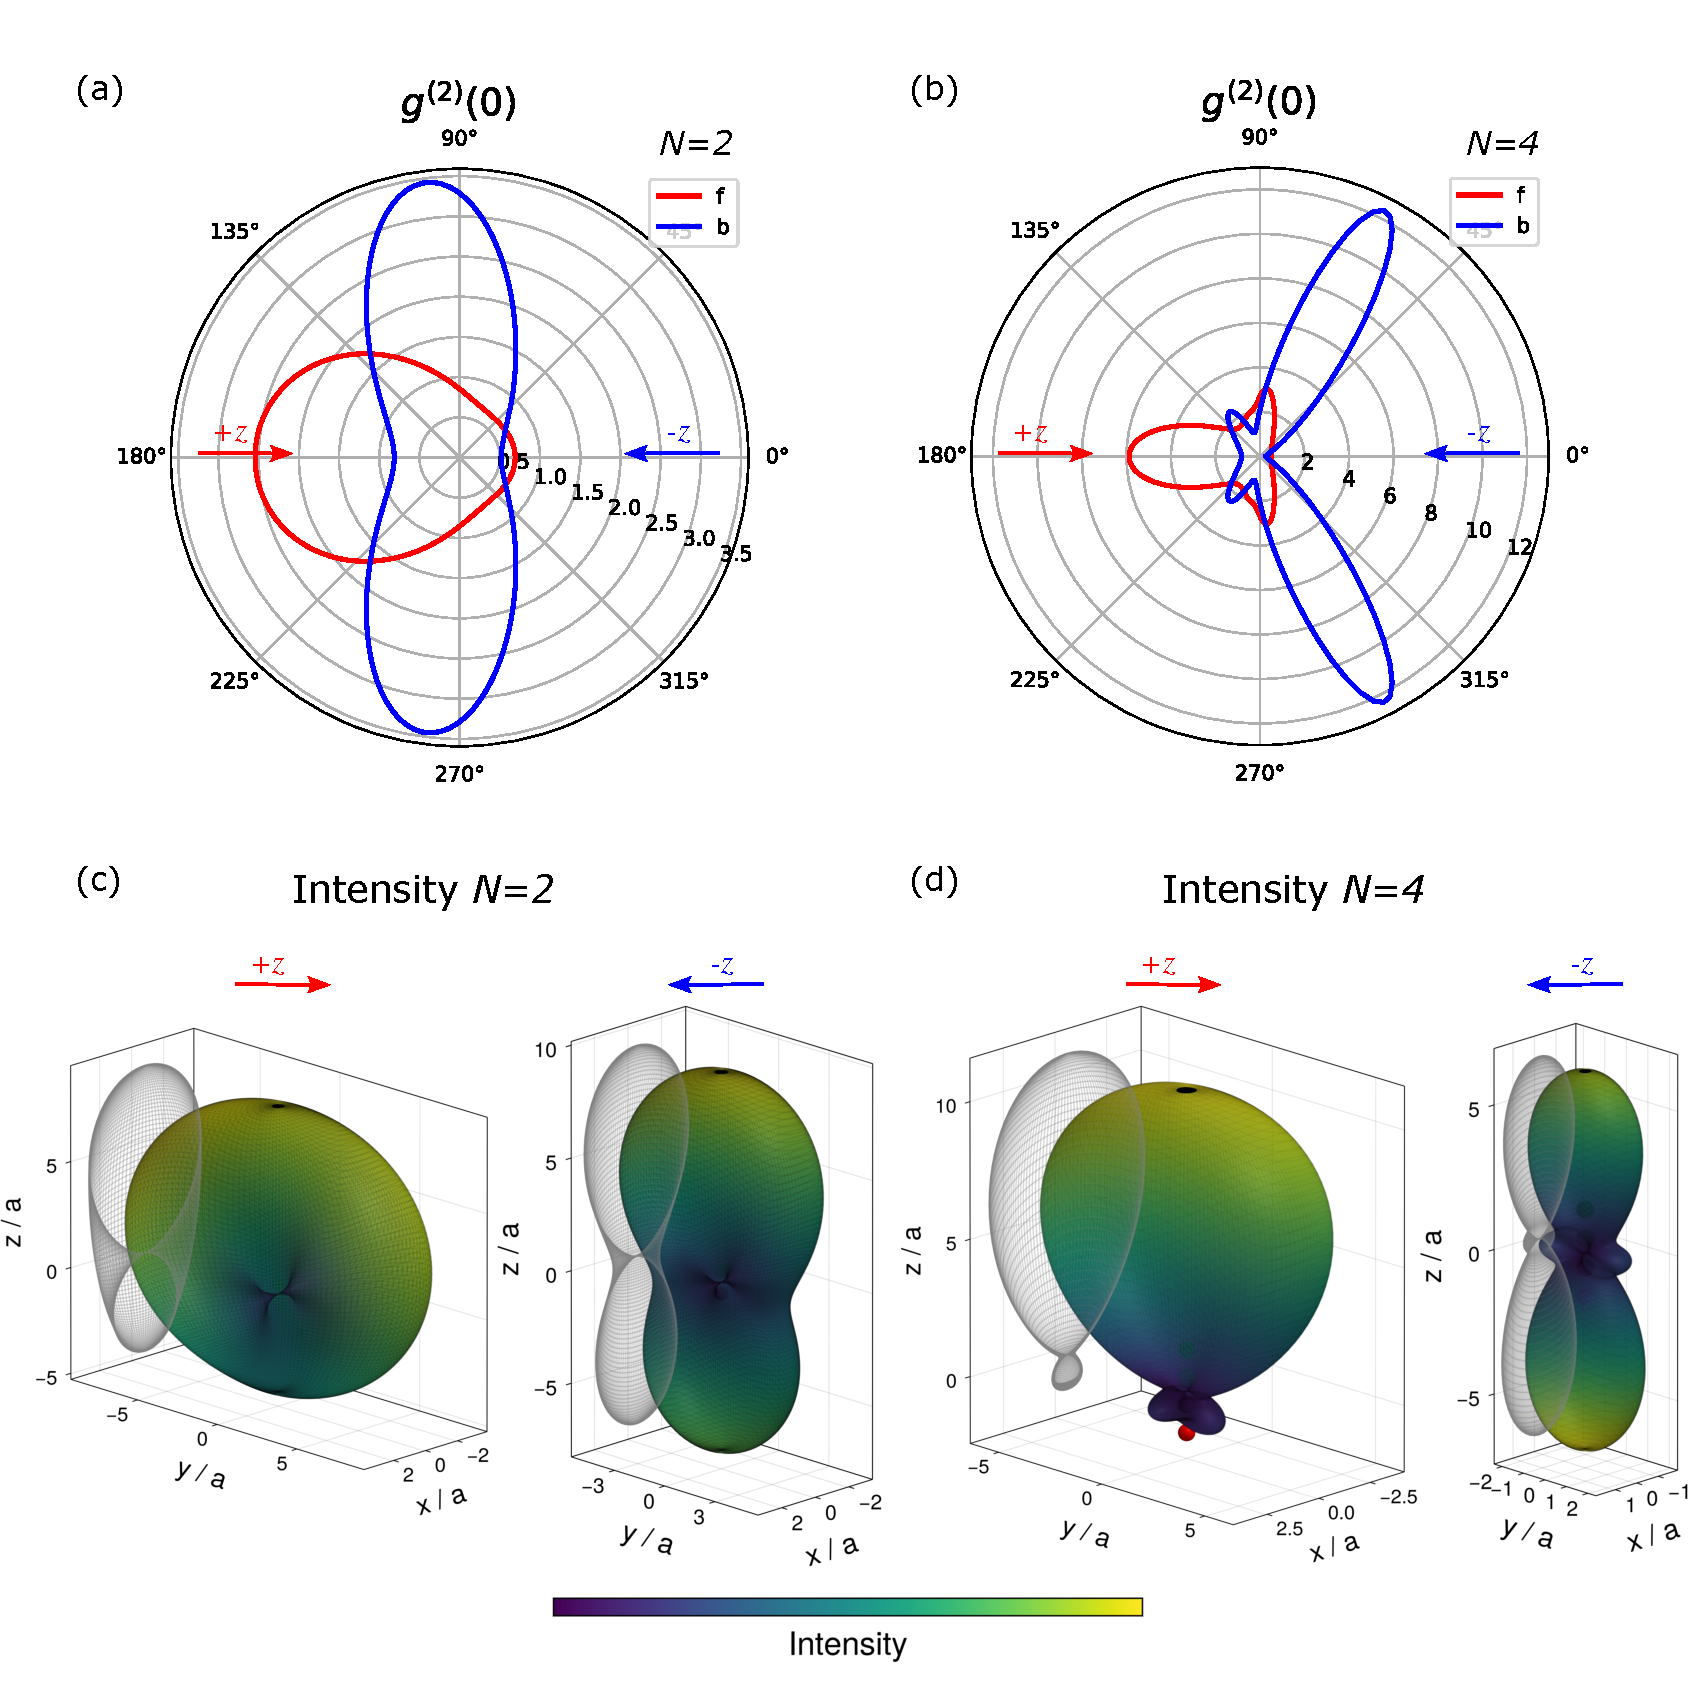
\includegraphics[width=0.98\linewidth]{fig_2}
%     \caption{Angular dependence of the second-order coherence function, $g^{(2)}(0)$, when the system is primerily at the dark (a) and bright (b) states for the forward and backward directions of excitation, as well as the radiation patterns for the system parameters mirroring the ones used for the $g^{(2)}(0)$
%     function computations (c-d). The parameters are the following: (a), (c) ; (b), (d) .}
%     \label{fig:02}
% \end{figure}
%
% Describe here that the system behaviour including not only the scattering, but also the statistical properties strongly depends on the direction of excitation. 
% And choosing the agle where to put the detector, one can switch the statistical character of the emission from bunching behaviour to antibunching. 
% Realising the manipulation of the emission statistics from the system by demand. 
%
% This behaviour is closely connected to the populating the collective states like $|D\rangle$ and $|B\rangle$.
% It turns out that for particular parameters $|D\rangle$ and $|B\rangle$ states may switch, and at the end, we look at the most slowly decaying state.
%
% However, to understand better what happens in the system when we switch the direction of excitation, we need to consider the evolution of the system in more detail. 
% For this, we will use the formalism of quantum trajectories [Carmichael works] to unravel the system evolution obeying the master equation (\ref{eq:01}).
%

\section{Second-order coherence function for directed-detection operators}

Let us examine the expression for the second-order coherence function $g^{(2)}$, as defined in equation~(\ref{eq:05}). This expression quantifies the degree of coherence of the field scattered from the atomic array at two distinct points in space and time. Physically, it is interpreted as the interaction of two detectors positioned at points $\mathbf{R}_1$ and $\mathbf{R}_2$, measuring the signal from the array at times $t_1$ and $t_2$.

The expression in equation~(\ref{eq:06}) involves the operators of the scattered field, which depend explicitly on the dyadic Green tensor of the environment and encompass a summation over all atoms in the array. In this form, computing the correlation functions within the $g^{(2)}$ function can be challenging. To simplify our analysis, we restrict ourselves to the far-field approximation, where the detectors are situated much farther from the array than the wavelength of the scattered field and the geometric size of the array, i.e., $ |\mathbf{R}_j| \gg \lambda_0, N a$, where $j$ is the index of the detector.

To account for photons emitted in a specific direction $\bar{\mathbf{R}}(\theta, \varphi) = \mathbf{R} / R$, where $\mathbf{R}$ is the detector's coordinate and $R = |\mathbf{R}|$ (see Fig.~\ref{fig:01}), and detected within the solid angle element $d \Omega$ in the far field, we follow Ref.~\cite{carmichael2000quantum} and introduce the direct detection operators:
\begin{equation}
    \hat{S}(\theta, \varphi) = \sqrt{\frac{2 \epsilon_0 c}{\hbar \omega_0} \left( R^2 d \Omega \right)} \hat{E}_\mathrm{sc}^+ (\mathbf{R}(\theta, \varphi), t),
    \label{eq:12}
\end{equation}
where the operator of the scattered field in the far field takes the form:
\begin{align}
    \label{eq:13}
    &\hat{E}_\mathrm{sc}^+ (\mathbf{r}, t) = \frac{3 \hbar \gamma_0}{4 d k_0} \frac{\sqrt{1 - \left( \bar{\mathbf{d}} \cdot \bar{\mathbf{r}}^2 \right)}}{|\mathbf{r}|} \sum_{j=1}^N e^{-i k_0 \bar{\mathbf{r}} \cdot \mathbf{r}_j} \hat{\sigma}_j(t), \\
    & \bar{\mathbf{d}} = \frac{\mathbf{d}}{d}, \;\; \bar{\mathbf{r}} = \frac{\mathbf{r}}{|\mathbf{r}|} \nonumber
\end{align}
and $\mathbf{r}_j$ denotes the coordinate of the $j$-th atom. By substituting equation~(\ref{eq:13}) into equation~(\ref{eq:12}) and transitioning to spherical coordinates, we arrive at the simplified form of the directed-detection operator:
\begin{equation}
    \hat{S}(\theta, \varphi) = \sqrt{\gamma_0 D(\theta, \varphi) d \Omega} \sum_{j=1}^N e^{-i k_0 \bar{\mathbf{r}}(\theta, \varphi) \cdot \mathbf{r}_j} \hat{\sigma}_j,
    \label{eq:14}
\end{equation}
where 
\begin{equation}
    D(\theta, \varphi) = \frac{3}{8 \pi} \left[ 1 - \left( \bar{\mathbf{d}} \cdot \bar{\mathbf{r}}(\theta, \varphi) \right)^2 \right]
    \label{eq:15}
\end{equation}
is the dipole radiation pattern for emission from an individual atom.

Notably, the dissipative part of the master equation (\ref{eq:01}) can be expressed in terms of the directed-detection operators (\ref{eq:14}), which provides a clear physical interpretation of detecting scattered photons emitted by the atomic array in the direction $(\theta, \varphi)$. Thus, the dissipative part takes the following form:
\begin{align}
    \label{eq:16}
    \mathcal{D}_S(\cdot) = \frac{1}{2} \int d \Omega & \left( 2 \hat{S}(\theta, \varphi) \cdot \hat{S}^\dagger(\theta, \varphi) - \right. \\
                                                   & \;\; \left. \hat{S}^\dagger(\theta, \varphi)\hat{S}(\theta, \varphi) \cdot - \cdot \hat{S}^\dagger(\theta, \varphi) \hat{S}(\theta, \varphi)\right) \nonumber
\end{align}

We can now rewrite the $g^{(2)}$ function in terms of the operators $\hat{S}(\theta, \varphi)$. It takes the form:
\begin{equation}
    \label{eq:17}
    g^{(2)}(0) = \frac{\langle \hat{S}^\dagger(\theta, \varphi)\hat{S}^\dagger(\theta, \varphi)\hat{S}(\theta, \varphi)\hat{S}(\theta, \varphi) \rangle}{\langle \hat{S}^\dagger(\theta, \varphi)\hat{S}(\theta, \varphi) \rangle^2}
\end{equation}
From this equation, we can compute the second-order coherence function in the far field, depending on the angles $\theta$ and $\varphi$. Due to the axial symmetry of the system along the $z$-axis (see Fig.~\ref{fig:01}), we can focus solely on the $\theta$ dependence of the $g^{(2)}(0)$ function at a fixed $\varphi$ angle.

To compute the coherence function, we choose system parameters such that the most populated state is either the dark state (\ref{eq:11a}) or the bright state (\ref{eq:11b}), indicating that the system is in a collective state when excited from one direction. Simultaneously, we calculate the radiation pattern of the emission (i.e., the number of emitted photons as a function of the angles) for parameters that maximize the population of the dark or bright states. Figure~\ref{fig:02} illustrates the angular dependence of the $g^{(2)}(0)$ function alongside the emission intensity.

\begin{figure}[h]
    \centering
    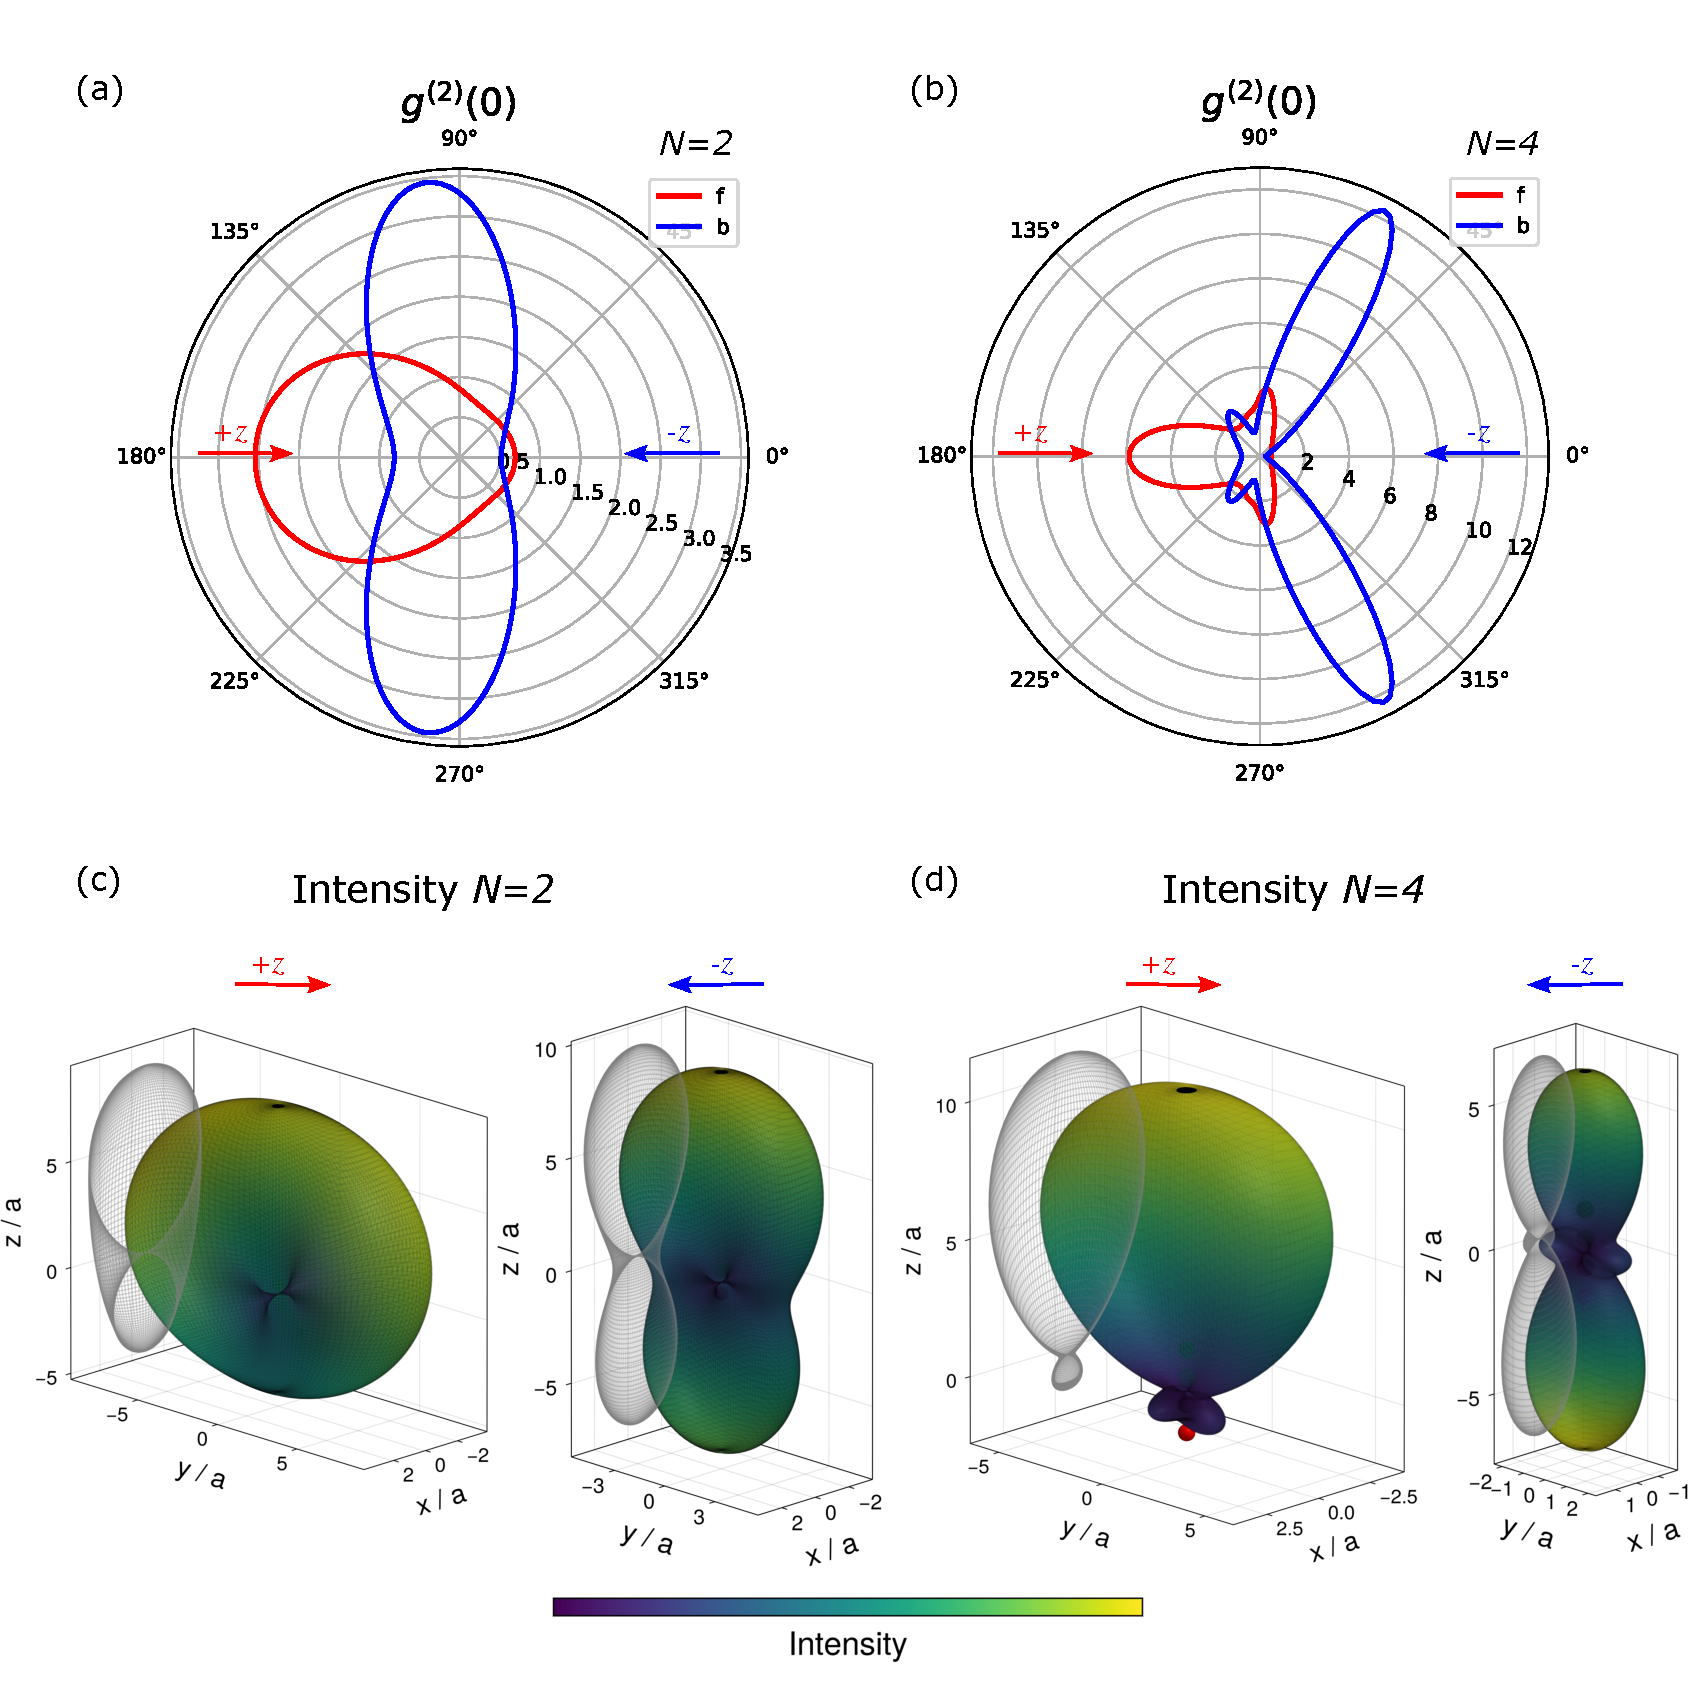
\includegraphics[width=0.98\linewidth]{fig_2}
    \caption{Angular dependence of the second-order coherence function, $g^{(2)}(0)$, when the system is primarily in the dark state for the two atom chain (a) and for the four atom chain (b) for the forward and backward excitation directions, along with the radiation patterns corresponding to the
    parameters used for the $g^{(2)}(0)$ function computations (c-d). The parameters optimizing the total scattering cross section are as follows: (a), (c) ; (b), (d).}
    \label{fig:02}
\end{figure}

The behavior of the system, including both the scattering dynamics and the statistical properties, is strongly influenced by the direction of excitation. By judiciously selecting the angle at which the detector is positioned, one can manipulate the statistical character of the emitted light,
transitioning between bunching and antibunching behavior. This capability to control the emission statistics on demand is closely linked to the occupation of collective slowly decaying state, namely dark state $|D\rangle$.

Interestingly, for certain parameter regimes, the states $|D\rangle$ and $|B\rangle$ can exchange roles, revealing a dynamic interplay among the collective excitations. This interplay highlights the nontrivial nature of photon emission from the atomic array, where the statistics can shift dramatically depending on the excitation conditions.

Ultimately, this exploration allows us to identify the state exhibiting the slowest decay rate, providing insights into the system's resilience under various excitation conditions. To deepen our understanding of the system's evolution as we vary the excitation direction, we turn to the formalism of
quantum trajectories, as described in the works [Carmichael]. This approach enables us to unravel the dynamics governed by the master equation (\ref{eq:01}), offering a comprehensive view of how collective states evolve in response to different excitation scenarios. By employing this formalism, we can analyze how the system transitions between states, providing a clearer picture of the underlying physics that dictate the observed coherence properties.

% \section{Collective jump operators and waiting time distributions}
%
% Following Carmichael works~\cite{carmichael2009statistical,carmichael2000quantum,clemens2003collective}, we can expand the reduced density operator of the system as a series of scattering records, i.e. the sequence of detection events that track a quantum system's interaction with its environment as
% $\hat{\rho}(t) = \sum_{\mathrm{rec}} P(\mathrm{rec}) | \psi_c (t) \rangle \langle  \psi_c (t) | $, where $\mathrm{rec}$ is the record denoting a particular sequence of photon detections (emissions), up to time t.
% The state $| \psi_c(t) \rangle = | \bar{\psi}_c(t) \rangle / \sqrt{\langle \bar{\psi}_c(t) | \bar{\psi}_c(t) \rangle}$ the normalized of the atoms conditioned on the occurrence of the sequence $\mathrm{rec}$, and $\bar{\psi}_c(t)$ is an unnormalized state of the atoms conditioned on $\mathrm{rec}$.
% $P(\mathrm{rec}) = \langle \bar{\psi}_c(t) | \bar{\psi}_c(t) \rangle$ is a probability to the particular scattering record to occur, so, obviously, $\sum_\mathrm{rec} P(\mathrm{rec}) = 1$.
% As shown in Ref.~\cite{carmichael2000quantum}, it is possible to construct such $| \psi_c(t) \rangle$ that the expansion holds with $\hat{\rho}(t)$ satisfying master equation (\ref{eq:01}) and $P(\mathrm{rec})$ gives the correct frequency of occurrence for every conceivable record. 
% The time evolution of $| \bar{\psi}_c(t) \rangle$ is generated by an effective non-Hermitian Hamiltonian
% \begin{equation}
%     \hat{H}_\mathrm{eff} = \hat{H}_S - i \hbar \sum_j \hat{O}_j^\dagger \hat{O}_j,
% \end{equation}
% and punctuated by jumps generated by a set of jump operators, $\hat{O}_j$ at the times of photon emissions.
% In our case, the role of jump operators may play directed-detection operators $\hat{S}(\theta, \varphi)$ (\ref{eq:14}) or the source-mode operators $\hat{J}_m$.
% The evolution is governed by the nonunitary Schrodinger equation with Hamiltonian $\hat{H}_\mathrm{eff}$.
%
% This time evolution can be simulated using Monte-Carlo method, see Ref.~\cite{carmichael2009statistical}. 
% Formally, the unnormalized state $| \bar{\psi}_c(t) \rangle$ for $n$ record events can be written as:
% \begin{align} 
%     | \bar{\psi}_c(t) \rangle =& \hat{B}(t - t_n) \hat{O}_n \hat{B}(t_n - t_{n-1}) \nonumber \\ 
%                                & \times \hat{O}_{n-1} \ldots \hat{O}_1 \hat{B}(t_1) |\psi(0) \rangle
%     \label{eq:18}
% \end{align}
% where operator $\hat{B}(t) = \exp(-i \hat{H}_\mathrm{eff} t / \hbar)$ describes the system evolution without jumps.
% Operator $\hat{O}_n$ is the operator responsible for the $n$th jump, which belongs to the set of jump operators of our choice, $\hat{O}_n \in \{\hat{O}_j\}$.
%
% \textit{
% Add a paragraph about the waiting time distribution (WTD) that can be obtained from Monte-Carlo simulation and its connection with the statistics of the emission. 
% Write about the importance of knowing WTD and what new information we can get from WTD in comparison with typical coherence functions.
% Add figs with WTD and g2 for source mode operators in the case of two atom chain (Fig. 3) and four atom chain (Fig. 4). 
% Tell that WTD for operators together and for each operator separately is always smaller or equal to the corresponding g2 function for these operators.
% Point out the difference of the WTD for the direction of excitation: for one direction we clearly see the collective behaviour, i.e., WTD and g2 function is more than 1 (cite Masson and Asenjo-Garcia Nat. Comm.); whereas for the other direction of excitation we mostly see the individual dynamics of atoms in the system, see Fig. 3, where the backward direction of excitation demonstrates more collective properties, and the forward direction of excitation demonstrates individual behaviour of the atoms in the chain. This behaviour and difference become more pronounced when we increase the number of atoms in the system, see Fig. 4 for the chain of four atoms.
% In particular, the behaviour of the WTDs related to each collective source mode operator can be also interpereted from the point of the collective and individual behaviour of the atoms.
% This observation leads us to the conclusion that we not only change the statistical properties of the emission in the system by switching the direction of excitation, but also switch between individual behaviour of the system and collective behaviour.
% }
%
% \begin{figure}
%     \begin{center}
%         \includegraphics[width=0.95\columnwidth]{fig_3}
%     \end{center}
% \caption{Waiting time distributions and $g^{(2)}(0)$ functions (solid lines) for individual source mode operators and all of them for forward and backward directions of excitation in a case of the two atom chain. The operators $\hat{J}_j$ are sorted in the ascending order of corresponding decay rates, i.e. $\hat{J}_1$ corresponds to the dark state and $\hat{J}_N$ corresponds to the bright state. The black dashed line shows the Poisson distribution of the waiting time. Parameters are the same as in Fig.~\ref{fig:02}(a, c)}\label{fig:03}
% \end{figure}
%
% \begin{figure}
%     \begin{center}
%         \includegraphics[width=0.95\columnwidth]{fig_4}
%     \end{center}
%     \caption{Waiting time distributions and $g^{(2)}(0)$ functions (solid lines) for individual source mode operators and all of them for forward and backward directions of excitation in a case of the four atom chain. The operators $\hat{J}_j$ are sorted in the ascending order of corresponding decay rates, i.e. $\hat{J}_1$ corresponds to the dark state and $\hat{J}_N$ corresponds to the bright state. The black dashed line shows the Poisson distribution of the waiting time. Parameters are the same as in Fig.~\ref{fig:02}(b, d)}\label{fig:04}
% \end{figure}

\section{Collective jump operators and waiting time distributions}

Following Carmichael's works~\cite{carmichael2009statistical,carmichael2000quantum,clemens2003collective}, we can expand the reduced density operator of the system as a series of scattering records, i.e., the sequence of detection events that track a quantum system's interaction with its environment, as
\[
\hat{\rho}(t) = \sum_{\mathrm{rec}} P(\mathrm{rec}) | \psi_c (t) \rangle \langle  \psi_c (t) |,
\]
where $\mathrm{rec}$ is the record denoting a particular sequence of photon detections (emissions) up to time $ t $. The state $ | \psi_c(t) \rangle = | \bar{\psi}_c(t) \rangle / \sqrt{\langle \bar{\psi}_c(t) | \bar{\psi}_c(t) \rangle} $ is the normalized state of the atoms conditioned on the occurrence of the sequence $ \mathrm{rec} $, and $ \bar{\psi}_c(t) $ is an unnormalized state of the atoms conditioned on $ \mathrm{rec} $. The probability $ P(\mathrm{rec}) = \langle \bar{\psi}_c(t) | \bar{\psi}_c(t) \rangle $ corresponds to a particular scattering record, satisfying $ \sum_\mathrm{rec} P(\mathrm{rec}) = 1 $. As shown in Ref.~\cite{carmichael2000quantum}, we can construct such $ | \psi_c(t) \rangle $ that the expansion holds with $ \hat{\rho}(t) $ satisfying the master equation (\ref{eq:01}), and $ P(\mathrm{rec}) $ gives the correct frequency of occurrence for every conceivable record.

The time evolution of $ | \bar{\psi}_c(t) \rangle $ is generated by an effective non-Hermitian Hamiltonian:
\begin{equation}
    \hat{H}_\mathrm{eff} = \hat{H}_S - i \hbar \sum_j \hat{O}_j^\dagger \hat{O}_j,
\end{equation}
and is punctuated by jumps generated by a set of jump operators $ \hat{O}_j $ at the times of photon emissions. In our case, the jump operators may be directed-detection operators $ \hat{S}(\theta, \varphi) $ (\ref{eq:14}) or the source-mode operators $ \hat{J}_m $. The evolution follows the non-unitary Schrödinger equation with Hamiltonian $ \hat{H}_\mathrm{eff} $.

This time evolution can be simulated using the Monte Carlo method, as described in Ref.~\cite{carmichael2009statistical}. Formally, the unnormalized state $ | \bar{\psi}_c(t) \rangle $ for $ n $ recorded events can be written as:
\begin{align} 
    | \bar{\psi}_c(t) \rangle = & \hat{B}(t - t_n) \hat{O}_n \hat{B}(t_n - t_{n-1}) \nonumber \\ 
                                & \times \hat{O}_{n-1} \ldots \hat{O}_1 \hat{B}(t_1) |\psi(0) \rangle
    \label{eq:18}
\end{align}
where $ \hat{B}(t) = \exp(-i \hat{H}_\mathrm{eff} t / \hbar) $ describes the system evolution without jumps. Here, $ \hat{O}_n $ is the operator responsible for the $ n $th jump, belonging to the set of jump operators $ \{\hat{O}_j\} $.

The waiting time distribution (WTD) between photon emission events, which can be obtained from Monte Carlo simulations, provides valuable insight into the statistics of emission processes. Unlike traditional coherence functions, which primarily provide information on intensity correlations, the WTD offers a more granular view of emission timings, revealing dynamic properties related to both collective and individual atomic behaviors in the system.

\begin{figure}
    \begin{center}
        \includegraphics[width=0.95\columnwidth]{fig_3}
    \end{center}
\caption{Waiting time distributions and $g^{(2)}(0)$ functions (solid lines) for individual source mode operators and all of them for forward and backward directions of excitation in a case of the two atom chain. The operators $\hat{J}_j$ are sorted in the ascending order of corresponding decay rates, i.e., $\hat{J}_1$ corresponds to the dark state and $\hat{J}_N$ corresponds to the bright state. The black dashed line shows the Poisson distribution of the waiting time. Parameters are the same as in Fig.~\ref{fig:02}(a, c)}\label{fig:03}
\end{figure}

For example, in Fig.~\ref{fig:03} and Fig.~\ref{fig:04}, we show the WTD and $ g^{(2)}(\tau) $ functions for source mode operators in two-atom and four-atom chains, respectively. These distributions illustrate that the WTD for a given operator or combination of operators is always less than or equal to the corresponding $ g^{(2)} $ function for the same operator(s). This trend highlights that while coherence functions indicate photon bunching or antibunching properties, the WTD can capture finer details about the collective nature of the emission events.

In Fig.~\ref{fig:03}, the waiting time distributions (WTDs) reveal distinct temporal characteristics and correlations in the two-atom chain depending on the direction of excitation. 

In the \textit{forward direction}, the WTD associated with the $ \hat{J}_1 $ operator exhibits a sharp peak near $ \tau / \bar{\tau} = 0 $, indicative of strong photon bunching at short times. This sharp feature suggests that $ \hat{J}_1 $ contributes significantly to temporally correlated emissions
immediately following excitation. In contrast, the WTD for $ \hat{J}_2 $ starts close to 1 and gradually decays, reflecting weaker correlations and a lower tendency for bunching. The combined WTD for $ \sum \hat{J}_j $ starts below 1, indicating the absence of collective effects. Thus, forward excitation predominantly displays individual atomic emission characteristics, with $ \hat{J}_1 $ as the primary source of temporal correlations while $ \hat{J}_2 $ displays uncorrelated emissions.

In the \textit{backward direction}, both $ \hat{J}_1 $ and $ \hat{J}_2 $ show enhanced temporal correlations but with different time scales. The WTD for $ \hat{J}_2 $ has a sharp peak near $ \tau / \bar{\tau} = 0 $, similar to that of $ \hat{J}_1 $ in the forward case, indicating strong bunching at
very short times. $ \hat{J}_1 $, however, exhibits a smaller, delayed peak, suggesting a distinct time scale of emission likely due to interference between atomic contributions. This delay introduces a second correlation peak and highlights the role of interference effects in shaping the emission
dynamics. The combined WTD $ \sum \hat{J}_j $ in the backward direction shows a significantly higher peak at the initial time than in the forward case, indicating pronounced collective behavior. The enhanced WTD implies that, in the backward direction, photon emissions are strongly correlated in time, with both atoms contributing to collective bunching.

Overall, the direction-dependent WTDs illustrate that the backward excitation direction enhances collective effects through constructive interference, leading to pronounced bunching and temporal correlations. The observed peaks in the WTDs of $ \hat{J}_1 $ and $ \hat{J}_2 $ reveal how individual atomic contributions interact differently under directional excitation for the collective source modes, with backward excitation allowing for a more substantial interplay between the atomic operators.

\begin{figure}
    \begin{center}
        \includegraphics[width=0.95\columnwidth]{fig_4}
    \end{center}
    \caption{Waiting time distributions and $g^{(2)}(0)$ functions (solid lines) for individual source mode operators and all of them for forward and backward directions of excitation in a case of the four atom chain. The operators $\hat{J}_j$ are sorted in the ascending order of corresponding decay rates, i.e., $\hat{J}_1$ corresponds to the dark state and $\hat{J}_N$ corresponds to the bright state. The black dashed line shows the Poisson distribution of the waiting time. Parameters are the same as in Fig.~\ref{fig:02}(b, d)}\label{fig:04}
\end{figure}

Figure~\ref{fig:04} presents the waiting time distributions (WTDs) and second-order correlation functions $ g^{(2)}(0) $ for a larger scale of an array, a four-atom chain, in both forward and backward directions, highlighting the influence of increased atom number on collective behavior compared to the two-atom case shown in Fig.~\ref{fig:04}. The collective source mode operators $ \hat{J}_j $ are sorted by their decay rates, with $ \hat{J}_1 $ corresponding to the dark state and $ \hat{J}_N $ (here $ \hat{J}_4 $) to the brightest state.

In the \textit{backward direction}, the WTDs of $ \hat{J}_1 $ and $ \hat{J}_2 $ display features very close to Poisson distibution, which reflects the behavior of individual atoms.
While the WTDs and $g^{(2)}(\tau)$ of $ \hat{J}_1 $ and $ \hat{J}_2 $ demonstrate antibunching and bunching behaviour, respectively, the combined WTD for $ \sum \hat{J}_j $ shows individual behavior, close to Poisson distrubution, similar to that observed in the two-atom case, see Fig.~\ref{fig:03}.

similar to those observed in the two-atom case, with $ \hat{J}_1 $ showing a strong initial peak indicating photon bunching and $ \hat{J}_2 $ displaying weaker correlations. However, with four atoms, the WTDs for $ \hat{J}_3 $ and $ \hat{J}_4 $ introduce additional peaks, indicating the presence of more complex temporal correlations. The combined WTD for $ \sum \hat{J}_j $ now shows enhanced collective behavior, with contributions from multiple decay channels. This enhancement demonstrates that as the number of atoms increases, forward emission gradually incorporates a broader range of collective modes, leading to more intricate emission dynamics.

However, in the \textit{backward direction}, the collective effects become even more pronounced. The WTDs for each operator exhibit a clear separation of time scales, with $ \hat{J}_4 $ and $\hat{J}_3$ showing a prominent initial peak indicative of strong photon bunching, while $\hat{J}_2$ and $
\hat{J}_1 $ exhibit initial antibunching behavior and delayed correlations, but at different time scales. The backward combined WTD $ \sum \hat{J}_j $ shows a pronounced peak, underscoring a strong collective effect at the initial times. This peak is significantly sharper and more sustained than in the two-atom case, indicating that constructive interference between atomic emissions becomes more substantial with additional atoms.

Overall, the comparison with a two-atom case, Fig.~\ref{fig:03}, reveals that increasing the number of atoms amplifies collective behavior. The separation of decay channels by their WTDs reflects enhanced temporal correlations and complex interference effects, which are key signatures of collective emission in larger atomic chains.

Interestingly, the direction of excitation here plays a crucial role in determining the collective properties of the system. For example, when excitation propagates in the backward direction in a two-atom chain (see Fig.~\ref{fig:03}), we observe enhanced collective behavior, with both WTD and $ g^{(2)}$ values exceeding unity, consistent with previous findings~\cite{masson2022universality}. Conversely, forward-directed excitation largely exhibits individual atomic dynamics. This contrast becomes more pronounced as the number of atoms in the chain increases (see Fig.~\ref{fig:04} for the four-atom case), where the forward direction emphasizes collective emissions, while the backward direction reinforces individual atomic contributions.

The WTD analysis of each source mode operator also sheds light on the interplay between collective and individual dynamics of the atoms. This approach allows us to conclude that by merely switching the direction of excitation, we can toggle between regimes of individual atomic behavior and collective dynamics, at the same time significantly changing the angular pattern of the second-order coherence function, $g^{(2)}$.




\section{Conclusion}\label{sec:conclusion}





% Acknowledgements
\begin{acknowledgments}
This work has been partially supported by the Simons Foundation and the Air Force Office of Scientific Research MURI program.
\end{acknowledgments}

% References
\bibliographystyle{apsrev4-2}
\bibliography{refs}

% Table of contents entry (Note: ToC is not typical in revtex articles, but if needed for some reason, you can include it)
\begin{figure}
\textbf{Table of Contents}\\
\medskip
  \includegraphics{toc-image}
  \medskip
  \caption*{ToC Entry}
\end{figure}

\end{document}
